\documentclass[11pt,a4paper]{article}
\usepackage[T1]{fontenc}
\usepackage[utf8]{inputenc}
\usepackage{lmodern}
\usepackage{amsmath,amssymb,amsthm,mathtools,mathrsfs}
\usepackage{graphicx,float,xcolor,multicol}
\usepackage[shortlabels]{enumitem}
\usepackage[margin=27mm]{geometry}
\usepackage{microtype,needspace,placeins}
\usepackage{tikz,tikz-cd}
\usetikzlibrary{arrows.meta,calc,positioning,patterns,decorations.pathreplacing}
\usepackage[colorlinks=true,linkcolor=teal,urlcolor=teal,citecolor=teal]{hyperref}
\setlength{\parindent}{0pt}
\setlength{\parskip}{.6em}
\setcounter{secnumdepth}{0}
\allowdisplaybreaks
\raggedbottom
\providecommand{\cross}{\times}
\DeclareUnicodeCharacter{2020}{\ensuremath{\dagger}}
\DeclareMathOperator{\supp}{supp}
\DeclareMathOperator*{\esssup}{ess\,sup}
\providecommand{\chapter}{\section}
\newenvironment{tool}[2]{\subsection*{Tool #1 --- #2}}{}
\newcommand{\ToolRef}[1]{Tool #1}
\newcommand{\FigureTag}[2]{\textit{Figure #1}}
\newcommand{\Result}[1]{\subsection*{#1}}
\newcommand{\Application}[1]{\subsubsection*{Application\if\relax\detokenize{#1}\relax\else\space--- #1\fi}}
\newcommand{\ProofHeading}{\par\textit{Proof.}\space}
\newcommand{\ProofOf}[1]{\par\textit{Proof of #1.}\space}
\newcommand{\RemarkHeading}{\par\textbf{Remark.}\space}
\newcommand{\NoteHeading}{\par\textbf{Note.}\space}
\newcommand{\ExerciseHeading}{\par\textbf{Exercise.}\space}

\graphicspath{{figures/complex-analysis/}}
\begin{document}
\section*{Rouché's Theorem and Bloch's Theorem}
% BLOG-CONTENT-BEGIN
% BLOG-PASSAGE: rouche-and-bloch:p0001
\subsection*{Tool 26 — Argument Principle}
\label{tool:argument-principle}

% BLOG-PASSAGE: rouche-and-bloch:p0002
\[
  \frac{1}{2\pi i}\int_\gamma\frac{f'(z)}{f(z)}\,dz
  =\#\{\text{zeros}\}-\#\{\text{poles}\}
\]
with multiplicities, in $\operatorname{int}(\gamma)$.

% BLOG-PASSAGE: rouche-and-bloch:p0003

\textit{Proof.}
It is rather trivial via the residue theorem. Tool 26 provides a substitute for the residue theorem.

% BLOG-PASSAGE: rouche-and-bloch:p0004

\subsection*{Hurwitz's Theorem}

% BLOG-PASSAGE: rouche-and-bloch:p0005
Let $\{f_n\}$ be such that $f_n\in H(U)$, where $U$ is a domain. If the $f_n$ are injective and $f_n\to f$ uniformly on compact sets, then $f$ is injective or constant.

% BLOG-PASSAGE: rouche-and-bloch:p0006
\textit{Proof.}
Assume that $f$ is nonconstant.
Suppose $f$ is not injective. Then $f(z)-f(z_0)$ has more than one zero. Since $f_n\to f$ uniformly, $f_n'\to f'$ uniformly; hence \(f_n-f_n(z_0)\longrightarrow f-f(z_0)\)
and
\[
  \bigl(f_n-f_n(z_0)\bigr)'
  \longrightarrow \bigl(f-f(z_0)\bigr)'.
\]
Therefore,
\[
  \frac{1}{2\pi i}\int_{C_\varepsilon(z_0)}
  \frac{(f_n-f_n(z_0))'}{f_n-f_n(z_0)}\,dz
  \longrightarrow
  \frac{1}{2\pi i}\int_{C_\varepsilon(z_0)}
  \frac{(f-f(z_0))'}{f-f(z_0)}\,dz.
\]
A sequence of $1$'s converges to something greater than $1$, a contradiction.

% BLOG-PASSAGE: rouche-and-bloch:p0007
\subsection*{Residue at infinity}
The residue at $\infty$ is not $a_{-1}$ of the expansion of $f(1/z)$; surprisingly, it is $-a_1$. Let us define the pole at $\infty$ by analogy:
\[
  \frac{1}{2\pi i}\int_{\partial\overline{B_R(0)}+z_0}
  f(z-z_0)\,d(z-z_0)=\operatorname{Res}(f;z_0).
\]
Under the inversion $z\mapsto1/z$,
\begin{align*}
  \frac{1}{2\pi i}\int_{\partial\overline{B_\varepsilon(0)}}
  f(1/z)\,d(1/z)
  &=\operatorname{Res}(f;\infty)\\
  &=-\frac{1}{2\pi i}\int_{\partial\overline{B_\varepsilon(0)}}
  f(1/z)\frac{1}{z^2}\,dz\\
  &=-\operatorname{Res}\!\left(\frac{f(1/z)}{z^2};0\right)
  =-a_1.
\end{align*}
For a meromorphic function on the Riemann sphere, one has
\[
  \operatorname{Res}(f;\infty)
  =-\sum_{z\in\mathbb C}\operatorname{Res}(f;z).
\]

% BLOG-PASSAGE: rouche-and-bloch:p0008

\subsection*{Tool 27 — Rouch\'e's Theorem}

% BLOG-PASSAGE: rouche-and-bloch:p0009
Let $\gamma$ be a Jordan curve such that \(\operatorname{int}(\gamma)\cup\gamma^*\subset U,\)
and let $f,g\in H(U)$. If
\[
  |g(z)|<|f(z)|\qquad(z\in\gamma^*),
\]
then $f$ and $f+g$ have the same number of zeros in $\operatorname{int}(\gamma)$.

% BLOG-PASSAGE: rouche-and-bloch:p0010

Indeed, note that
\[
  f+sg\ne0\quad\text{on }\gamma^*,
  \qquad s\in[0,1],
\]
and
\[
  \frac{1}{2\pi i}\int_\gamma\frac{(f+sg)'}{f+sg}\,dz
\]
is continuous in $s$. Hence the number of zeros of $f+sg$ in $\operatorname{int}(\gamma)$ is constant.

% BLOG-PASSAGE: rouche-and-bloch:p0011
Let $f,g\in H(\overline{B_1(0)})$. If $f$ has a simple zero, then, for $\varepsilon$ small enough, $f+\varepsilon g$ has a unique zero in $B_1(0)$. Consider the map $\varepsilon\mapsto z_\varepsilon$, where $z_\varepsilon$ is that zero. The map is continuous, since

% BLOG-PASSAGE: rouche-and-bloch:p0012
\[
  z_\varepsilon
  =\frac{1}{2\pi i}\int_{\partial B_\delta(0)}
  z\,\frac{f_\varepsilon'(z)}{f_\varepsilon(z)}\,dz
\]
is continuous in $\varepsilon$. Pretty cool, right? The continuous deformation of holomorphic functions also deforms their zeros continuously, as long as the map $\varepsilon\mapsto z_\varepsilon$ is well-defined.

% BLOG-PASSAGE: rouche-and-bloch:p0013
\subsection*{Open Mapping Theorem}

% BLOG-PASSAGE: rouche-and-bloch:p0014
If $f\in H(U)$, then $f$ is an open map.

% BLOG-PASSAGE: rouche-and-bloch:p0015
\textit{Proof.}
Consider $f(z)-f(z_0)$ on a ball $B_\varepsilon(z_0)$ such that \(\#\{z:f(z)=f(z_0),\ z\in\overline{B_\varepsilon(z_0)}\}=1.\)
The set $f(\partial B_\varepsilon(z_0))$ is compact and
\[
  f(\partial B_\varepsilon(z_0))\cap\{f(z_0)\}=\varnothing.
\]
Let
\[
  d=\operatorname{dist}\bigl(f(\partial B_\varepsilon(z_0)),f(z_0)\bigr).
\]
If $|w-f(z_0)|<d/4$, then
\[
  |f(z)-f(z_0)|>|w-f(z_0)|
  \qquad(z\in\partial B_\varepsilon(z_0)).
\]
Hence $f(z)-w$ has a zero in $B_\varepsilon(z_0)$.

% BLOG-PASSAGE: rouche-and-bloch:p0016
\subsection*{Inverse Function Theorem}

% BLOG-PASSAGE: rouche-and-bloch:p0017
Let $f\in H(U)$. If $f'(z_0)\ne0$, then there exists a neighborhood $V$ of $z_0$ in $U$ such that \(f:V\to f(V)\)
is a complex diffeomorphism.

% BLOG-PASSAGE: rouche-and-bloch:p0018
\textit{Proof.}
Write
\[
  f(z)-w=(f(z_0)-w)
  +(z-z_0)\left(\sum_{n\ge0}f^{(n+1)}(z_0)(z-z_0)^n\right).
\]
Let
\[
  g(z)=(z-z_0)\left(\sum_{n\ge0}f^{(n+1)}(z_0)(z-z_0)^n\right).
\]
Then $g$ has a simple zero at $z_0$. Let $h(z)=f(z_0)-w$. Then, as $z\to z_0$, $g(z)\to0$. In fact, there exists $\varepsilon$ such that, if $|z-z_0|<\varepsilon$, then $|g(z)|<|f(z_0)-w|$. Thus, in $B_{\varepsilon/2}(z_0)$, $f(z)-w$ has no root.

% BLOG-PASSAGE: rouche-and-bloch:p0019
Oops, I made a mistake! Do not make the mistake of swapping $f$ and $g$ in Rouch\'e's theorem.

% BLOG-PASSAGE: rouche-and-bloch:p0020
The proof again: write \(f(z)-w=(f(z_0)-w)+g(z),\) and choose $\varepsilon>0$ so that $z_0$ is the only zero of $g$ in $\overline{B_\varepsilon(z_0)}$ and $f'(z)\ne0$ there. Put
\[
  \min_{z\in\partial B_\varepsilon(z_0)}|g(z)|=:g_0>0.
\]
Then, if $w\in B_{g_0}(f(z_0))$, Rouch\'e's theorem shows that $f(z)-w$ has exactly one zero in $B_\varepsilon(z_0)$; it is simple because $f'$ does not vanish there. Let
\[
  V=B_\varepsilon(z_0)\cap f^{-1}\bigl(B_{g_0}(f(z_0))\bigr).
\]
The inverse is therefore well-defined on $B_{g_0}(f(z_0))$, and
\[
  \lim_{h\to0}
  \frac{f^{-1}(z+h)-f^{-1}(z)}{h}
  =\frac{1}{f'(f^{-1}(z))}.
\]

% BLOG-PASSAGE: rouche-and-bloch:p0021
\textbf{Remark.}
Observe that the simplicity of the proof uses the full strength of holomorphicity. Contrast it with the proof of the real-variable inverse function theorem.

% BLOG-PASSAGE: rouche-and-bloch:p0022
\paragraph{Important remark.}
Using the same idea, if $f(z)-f(z_0)$ has a zero at $z_0$ of order $k$, then argue as before with the local expansion
\[
  f(z)-w=(f(z_0)-w)
  +(z-z_0)^k u(z),\qquad u(z_0)\ne0,
\]
to conclude that, locally, \(f:V\to f(V)\) is a $k$-fold covering holomorphic map. Notice that this is the complex analogue of the rank theorem for the case of Fr\'echet differentiable functions in $\mathbb R^n$.

% BLOG-PASSAGE: rouche-and-bloch:p0023
\subsection*{Tool 28 — Geometric Series}

% BLOG-PASSAGE: rouche-and-bloch:p0024
\[
  \frac{1}{1-z}=\sum_{n\ge0}z^n.
\]

% BLOG-PASSAGE: rouche-and-bloch:p0025
Although this might seem innocuous, one must see Tool $28$ in action to appreciate its reach; whatever it reaches is important in its own right.

% BLOG-PASSAGE: rouche-and-bloch:p0026
Let $f$ be meromorphic in $\overline{B_1(0)}$, with only a simple pole at $z_0$; that is,
\[
  f\in H\bigl(\overline{B_1(0)}\setminus\{z_0\}\bigr).
\]
Consider the Laurent series locally at $z_0$, and let
\[
  f(z)=\sum_{n\ge0}a_nz^n
\]
be the Taylor series around $0$. Then
\[
  f(z)=\frac{c}{z-z_0}+h(z)
  =\frac{c}{z-z_0}+\sum_{n\ge0}b_n(z-z_0)^n
  =\sum_{n\ge0}a_nz^n.
\]
Expand $h(z)$, where $h\in H(U)$, around $0$:
\[
  h(z)=\sum c_nz^n.
\]
Now note that
\[
  \frac{c}{z-z_0}
  =-\frac{c/z_0}{1-z/z_0}
  =-\sum_{n\ge0}\frac{c}{z_0^{n+1}}z^n,
\]
so
\[
  a_n=c_n-\frac{c}{z_0^{n+1}},
  \qquad
  \frac{a_n}{a_{n+1}}
  =\frac{c_n-c/z_0^{n+1}}{c_{n+1}-c/z_0^{n+2}}.
\]
Consequently,

% BLOG-PASSAGE: rouche-and-bloch:p0027
\[
  \frac{a_n}{a_{n+1}}
  =z_0\left(\frac{c_nz_0^{n+1}-c}{c_{n+1}z_0^{n+2}-c}\right).
\]
Since $h(z)$ is convergent at $z_0$,
\[
  \lim_{n\to\infty}c_nz_0^{n+1}=0,
  \qquad
  \lim_{n\to\infty}\frac{a_n}{a_{n+1}}=z_0.
\]

% BLOG-PASSAGE: rouche-and-bloch:p0028
\textbf{Remark.} Thus the radius of convergence of a Taylor series is exactly equal to the distance to the nearest pole of $f$.

% BLOG-PASSAGE: rouche-and-bloch:p0029
\subsection*{Bloch's Theorem}

% BLOG-PASSAGE: rouche-and-bloch:p0030
Let \(f:D(z_0,R)\to\mathbb C\)
be holomorphic and $f'(z_0)\ne0$. There exist absolute constants $c',c''>0$ such that
\[
  f\bigl(B_R(z_0)\bigr)
  \supseteq B_{c'|f'(z_0)|R}(w_0)
\]
for some $w_0\in\mathbb C$.

% BLOG-PASSAGE: rouche-and-bloch:p0031

\textit{Proof.}
Apply the affine normalization
\[
  F(z):=\frac{f(Rz+z_0)-f(z_0)}{Rf'(z_0)}.
\]
Then \(F(0)=0\) and \(F'(0)=1\), so it is enough to prove the result for \(z_0=0\) and \(R=1\).
Assume \(|f'(z)|<2|f'(0)|=2.\)
By the \BlogPost{goursat-cauchy}{Cauchy estimate}, if
\[
  f(z)=\sum_{n\ge0}a_nz^n,
\]
then $|a_n|\le2$. Hence, with $a_0=0$,
\[
  |f(z)|\ge |z|-\left|\sum_{n\ge2}a_nz^n\right|
  \ge |z|-\frac{2|z|^2}{1-|z|}
  \qquad(z\in D(0,1)).
\]
The same estimate holds on $D(0,1/8)$. The function $|f(z)/z|$ attains its minimum on $\partial D(0,1/8)$, since $f$ has a simple zero at $0$. On $\partial D(0,1/8)$,
\begin{align*}
  |f(z)|
  &\ge \frac18-\frac{2(1/8)^2}{1-1/8}\\
  &=\frac18-\frac{2}{64}\cdot\frac87
   =\frac14\left(\frac12-\frac17\right)
   =\frac{5}{56}.
\end{align*}
Now let $|w|<5/56$ and put $g=-w$. On $\partial D(0,1/8)$, \(|f(z)|>|g|,\)
and hence $f-w$ has a zero, since $f$ has a simple zero. Therefore,
\[
  D\left(0,\frac{5}{56}\right)
  \subset f\bigl(D(0,1/8)\bigr)
  \subset f\bigl(D(0,1)\bigr).
\]
This proves that there exists an absolute constant $c'$ such that, if \(|f'(z)|<2|f'(z_0)|,\)
then
\[
  D\bigl(f(z_0),c'|f'(z_0)|R\bigr)
  \subset f\bigl(D(z_0,R)\bigr).
\]

% BLOG-PASSAGE: rouche-and-bloch:p0032
It remains to remove the additional hypothesis $|f'(z)|<2|f'(z_0)|$. If the hypothesis holds for $z\in D(z_0,R/4)$, then Bloch's theorem follows. Otherwise there exists
\[
  z_1\in D(z_0,R/4)
\]
such that
\[
  |f'(z_1)|>2|f'(z_0)|.
\]
Now replace $z_0$ by $z_1$ and $R$ by $R/2$, and note that with $z_0=0$,
\[
  |z_n|<\sum_{n\ge2}\frac{R}{2^n},
  \qquad
  |z_n|<\frac R2\quad(\forall n).
\]
Thus $z_n\to z_0'\in D(z_0,R)$ and \(|f'(z_n)|>2^n|f'(z_0)|.\)
Therefore, $f'(z)$ blows up at $z_0'$, a contradiction.

% BLOG-PASSAGE: rouche-and-bloch:p0033

\paragraph{Final remark.} We continue in \BlogPost{separation-and-holomorphic-lifting}{Separation by a Polygonal Path/Arc and Holomorphic Lifting} with some important constructions: a branch of a logarithm, a lift of a holomorphic map, biholomorphisms, and the Jordan curve theorem.
\begin{figure}[htbp]
  \centering
  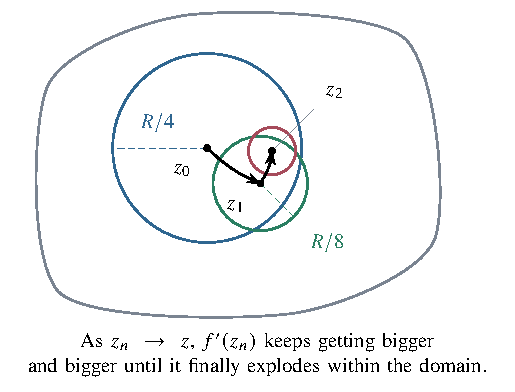
\includegraphics[width=0.72\textwidth]{note7-fig-05.pdf}
\end{figure}
% BLOG-CONTENT-END
\end{document}
